% peer_poll.tex
\chapter{Peer/Poll Processes}
\label{cha:peer/poll_processes}

\section{Definitions}%
\label{sec:peer/poll_concepts}
Before discussing peer/poll processes in this chapter, we need to go through
some definitions. Some of them may not be clear at this point, we will discuss
them with more detail later.
\begin{enumerate}
    \item Offset $\theta$\\
        The maximum-likelihood time offset of the server clock relative to the
        system clock. It describes how different the client's time
        and the server's time are.
        % $$\theta_{AB} = \frac{1}{2}\left[\left(T_{i-2} - T_{i-3}\right) +
        % \left(T_{i-1} - T_i\right)\right]$$
    \item Delay $\delta$\\
        The round-trip delay between the client and server. It is equal to the
        time that a massage travels from the client to the server plus the time
        it comes back.
        % $$\delta_{AB} = \left(T_{i} - T_{i-3}\right) - \left(T_{i-1} -
        % T_{i-2}\right)$$
    \item Dispersion $\varepsilon$\\
        The maximum error inherent in the measurement.
        Another definition: Potential clock offset error due to the maximum
        uncorrected system clock frequency error.
        These definitions are in some respect confused, we will discuss it with
        more detail in Section~\ref{sec:peer_processes}.
        % from website https://www.eecis.udel.edu/~mills/ntp/html/stats.html
    \item Jitter $\varphi$\\
        The root-mean-square (RMS) of a series of time offsets; this indicates 
        how stable the offset is.
\end{enumerate}

\section{Overview}%
\label{sec:peer_poll_overview}
Figure~\ref{fig:peer_poll_processes} shows the basic architecture of peer/poll
processes. The communication between client and server uses on-wire protocol,
which can provide sample statistics ($\theta_0, \delta_0, t_0$ in the figure).
The recent eight samples are stored in a shift register, with one more sample
statistic added ($\varepsilon$). Then peer process applies clock filter
algorithm, which generates peer statistics ($\theta, \delta, \varepsilon,
\varphi$ in the figure), and passes them to system process.


% figures/peer_poll_figure.tex

\begin{figure}[htpb]
\begin{center}
\begin{tikzpicture}[scale=0.7, transform shape,
        squarednode/.style={rectangle, draw=black, very thick, minimum
        size=10mm, minimum width=20mm, align=center},
        border/.style={draw=black, dashed, very thick},
    ]
    % Nodes
    % server
    \node[squarednode]  (s)                {Server};

    % on-wire protocol
    \node[align=center] (onwire) at ($(s.east) + (2.5, 2)$) {On-wire Protocol};
    \draw[border] ($(onwire.north west) + (-0.2, 0.2)$) -|
            ($(onwire.north east) + (0.2, -5)$) -|
            ($(onwire.north west) + (-0.2, 0.2)$);
    % poll process
    \node[squarednode] (poll) at ($(onwire) + (0, -6)$) {Poll Process};
    \draw[-latex, thick] (poll) |- ($(s.south) + (0, -0.5)$) -- (s);

    % shift registers
    \node[squarednode] (sr) at ($(onwire) + (4.5,-2)$) 
            {Shift Registers\\
            $(\theta_1, \delta_1, \varepsilon_1, t_1)$\\
            $(\theta_2, \delta_2, \varepsilon_2, t_2)$\\
            $(\theta_3, \delta_3, \varepsilon_3, t_3)$\\
            $(\theta_4, \delta_4, \varepsilon_4, t_4)$\\
            $(\theta_5, \delta_5, \varepsilon_5, t_5)$\\
            $(\theta_6, \delta_6, \varepsilon_6, t_6)$\\
            $(\theta_7, \delta_7, \varepsilon_7, t_7)$\\
            $(\theta_8, \delta_8, \varepsilon_8, t_8)$
            };
    \draw[-latex, thick] (s) -- (sr) node[midway, above] 
            {$(\theta_0, \delta_0, t_0)$};
    % clock filter algorithm
    \node[squarednode] (cf) [right=of sr] {Clock Filter\\ algorithm};
    \draw[-latex, thick] (sr) -- (cf);

    % peer process
    \node[align=center] (peer) [below=2mm of sr.south east] {Peer Process};
    \draw[border] ($(sr.north west) + (-0.5, 0.2)$) -- 
            ($(sr.south west) + (-0.5, -1.2)$)
            -|
            ($(cf.east) + (0.2, 0)$) |-
            ($(sr.north west) + (-0.5, 0.2)$);


    % system process
    \node[squarednode] (sp) [right=2.5 of cf] {System process};
    \draw[-latex, thick] (cf) -- (sp) node[midway, above] 
            {$(\theta, \delta, \varepsilon, \varphi)$};
    
    % synchronizations
    % \draw[-latex, ultra thick] (s1) -- (rc);

\end{tikzpicture}
\end{center}
\caption{Peer/Poll processes}
\label{fig:peer_poll_processes}
\end{figure}



% fig:peer_poll_processes

The purpose of peer processes is to communicate with servers and to calculate
and keep statistics of the communications which can be used to determine how
reliable the servers are. Poll processes are used to manage the communications
to get sufficient data without making the servers too busy.

\section{On wire protocol}%
\label{sec:on_wire_protocol}
In NTP subnet, a client can send a request to server and the server sends back
a response after it dealt with the request. The whole round of the
communication can generate a sample. For every sample, the client wants to know
the difference between the server's system clock and its, aka offset.  But it
may take a while for the server to give the response. And it is not
predictable, as well as the network delay between the two devices.  In NTP
subnet, clients and servers communicate under on-wire protocol. It provides a
smart way to calculate offset and delay for every sample. 

\subsection{Statistics calculation}%
\label{sub:statistics_calculation}
Figure~\ref{fig:on_wire1} represents the timestamps and communications between
a client and a server. The vertical dash line indicates the same time. The
arrow indicates the communication packets sent from one side and received at
the other side. The notation $T_i$ stands for the timestamp gotten from the
system clock of one device. 

% figures/on_wire1.tex

\begin{figure}[htpb]
\begin{center}
\begin{tikzpicture}[scale=0.7, transform shape,
        textnode/.style={rectangle, very thick, minimum
        size=10mm, minimum width=20mm, align=center},
        border/.style={draw=black, dashed, very thick},
        arrow/.style={-latex, ultra thick},
    ]
    % server
    \node[textnode]  (s)                {Server};
    \draw[arrow]     (s) -- ($(s) + (10,0)$);

    % client
    \node[textnode]  (c)    [below=20mm of s]            {Client};
    \draw[arrow]     (c) -- ($(c) + (10,0)$);

    % communications
    \draw[arrow]     ($(c) + (5, 0)$) -- ($(s) + (6, 0)$);
    \draw[arrow]     ($(s) + (8, 0)$) -- ($(c) + (9, 0)$);

    % vertical line
    \draw[border]    ($(s) + (3, 1)$) -- ($(c) + (3, -1)$);

    % labels
    \node[textnode] at ($(c) + (2.5, -0.5)$)   {$t_0$};
    \node[textnode] at ($(s) + (2.5, 0.5)$)    {$t_1$};
    \node[textnode] at ($(c) + (5, -0.5)$)   {$t_2$};
    \node[textnode] at ($(s) + (6, 0.5)$)    {$t_3$};
    \node[textnode] at ($(s) + (8, 0.5)$)    {$t_4$};
    \node[textnode] at ($(c) + (9, -0.5)$)   {$t_5$};

\end{tikzpicture}
\end{center}
\caption{Time stamps}
\label{fig:on_wire1}
\end{figure}



% fig:on_wire1

In ideal situation, if we have $T_1$ and $T_0$, which are timestamps gotten
from both devices at the same time, then we can get the offset $\theta$:
$$\theta = T_1 - T_0$$
However, we cannot do this since we cannot determine whether two timestamps
were token at the same time. The on-wire protocol actually calculates the
offset in an alternative way:
\begin{equation}
    \theta = \frac{1}{2}\left[(T_3 - T_2) + (T_4 - T_5)\right]
    \label{eq:offset_def}
\end{equation}
Note that this equation is equivalent to:
$$\theta = \frac{T_3 + T_4}{2} - \frac{T_2 + T_5}{2}$$
which means that the offset is equal to the difference between two timestamps
which are the middle points of $T_3, T_4$ and $T_2, T_5$. 
If the network delay is symmetric, which means the time for packets to travel
from client to server and the time for packets to get back are equal, the
middle points are at the same time. In this case, it is equivalent to the ideal
situation. If the delay is asymmetric, there will be an error of the
calculation. This error is impossible to be corrected. However, there is one
scenario that the error can be attenuated.~\cite{redbook} We will discuss this
part in Section~\ref{sub:huff_n_puff_filter}.

The delay $\delta$ is calculated by:
\begin{equation}
    \delta = (T_5 - T_2) - (T_4 - T_3)
    \label{eq:delay_def}
\end{equation}
It is actually a difference of two time periods. It is not impacted by the
offset, since each time period is calculated using two timestamps from the same
device. 

As mentioned in Section~\ref{sec:adjusting_system_time}, the frequency of 
system clock may not be accurate. It also impacts the calculations here. We
will discuss this more in Section~\ref{sec:phase_frequency_prediction} and
Section~\ref{sec:intrinsic_frequency_offset}.

There is another statistic $t$ in Figure~\ref{fig:peer_poll_processes}, which
indicates the time that the offset $\theta$ and delay $\delta$ are calculated.
In practice we can let $t = T_5$, because it is just used to indicate the order
of groups of sample statistics, we do not need it to be extremely accurate.
In Figure~\ref{fig:peer_poll_processes}, we add subscript 0 to distinguish the
new group of samples statistics and the groups which are in the shift register.

\subsection{Timestamps in NTP packet}%
\label{sub:timestamps_in_ntp_packet}
% how to store timestamps and modes
% https://www.eecis.udel.edu/~mills/onwire.html
NTP uses NTP packets in communications. The NTP packet is a UDP
datagram~\cite{rfc5905}. There are four timestamps in NTP packet header:
\begin{enumerate}
    \item Reference Timestamp\\
        Time when the system clock was last set or corrected.
    \item Origin Timestamp (\emph{org})\\
        Time at the client when the request packet departs from it.
    \item Receive Timestamp (\emph{rec})\\
        Time at the server when the request packet is receive by it.
    \item Transmit Timestamp (\emph{xmt})\\
        Time at the server when the response packet departs from it.
\end{enumerate}
In peer process, we are interested in another one: destination
timestamp(\emph{dst}), which is the time at the client when it receives the
response packet. And the reference timestamp is not interested here. In
Figure~\ref{fig:on_wire1}, the packet leave at $T_4$ contains $T_4, T_3$ and
$T_2$ in its header, where
$$ org = T_2,~rec = T_3,~xmt = T_4 $$
When the client gets the packet, it captures $dst = T_5$.

The purpose of on-wire protocol is to calculate offset $\theta$ and delay
$\delta$ based on the communication. The four timestamps used in
Equation~\ref{eq:offset_def} and Equation~\ref{eq:delay_def} are important,
which are \emph{org}, \emph{rec}, \emph{xmt} and \emph{dst}.
High accuracy requires that they are captured as close to the actual time of
the relative event (sending or receiving packet) as possible. On-wire protocol
provides two interleaved modes which are \emph{interleaved symmetric} and
\emph{interleaved broadcast}. They are extensions of basic symmetric mode and
basic broadcast mode.~\cite{on_wire} 
%
In basic modes, \emph{org} and \emph{xmt} in outgoing packet are captured
before the packet is made, which is not the timestamp when the packet is sent. 
This kind of timestamps are called \emph{softstamps}. In this case, 
after softstamp is captured, there are something else to do before sending the
packet, such as add validation information to the packet and adding the packet
to the output queue, then the packet will wait in the queue before it is sent.
For \emph{rec} and \emph{dst}, which are also called \emph{drivestamps}, they
are captured ``shortly after the input device interrupt and before adding the
buffer to the input queue''\cite{on_wire}. We can see that the drivestamps are
more accurate than softstamps because there is only a short delay by handling
the interrupt. If we can capture timestamps exactly when packets are sent or
received, they will be more accurate. However, we need additional hardware
support to do this.

In interleaved modes, we can make softstamps more accurate without
additional hardware support. The trade off is that we need more packets.
Instead of capturing softstamps before the packets are made, we can capture
them shortly after the output interrupt. In this case, the accuracy is similar
with drivestamps but they can not be sent in the very packets which they
represent the time they are sent. We need one more packet if we want to send
this kind of softstamps. More detail about interleaved modes are beyond the
scope of this thesis.

\subsection{Non-reliable protocol}%
\label{sub:non_reliable_protocol}
As mentioned in Section~\ref{sub:timestamps_in_ntp_packet}, the NTP packet is a
UDP datagram. This makes the on-wire protocol not reliable, which means that
there is no guarantee about the delivery of packets. Reliable delivery actually
decreases the reliability of NTP packets. Assume we are implementing on-wire
protocol to make it reliable by using similar technique like TCP, a lost packet
will be sent again. However, an identical packet is not valid since the
timestamp which indicates the time when the packet is sent is incorrect.

\section{Peer processes}%
\label{sec:peer_processes}
For each server, on-wire protocol provides sample statistics $\theta, \delta$
and $t$ and passes them to peer process. Then the peer process maintains them
and the clock filter algorithm calculates peer statistics based on them.

\subsection{Sample statistics maintenance}%
\label{sub:sample_statistics_maintenance}
As mentioned in Section~\ref{sec:peer_poll_overview}, there is a shift register
which stores the recent eight samples. When a packet arrives, the peer process
replace the oldest sample by the new one with a dispersion $\varepsilon$ added.
The dispersion is initialized as:
$$ \varepsilon = \rho_r + \rho_s + \phi (T_5 - T_2) $$
Where 
\begin{itemize}
    \item 
        $\rho_r$ is the root precision in NTP packet. 
    \item 
        $\rho_s$ is the system
        precision which we will discuss later.
    \item
        $\phi = 15 ppm = 15 \mu s/s$ is a constant.
    \item
        $T_5$ and $T_2$ are the two timestamps in Figure~\ref{fig:on_wire1}. In
        other word, $T_5$ is \emph{dst} and $T_2$ is \emph{org}.
\end{itemize}
After storing the sample statistics into the shift register, the dispersion
is increased in a constant rate $\phi$. 

The system precision is automatically determined by NTP, it represents the ``
the smallest possible increase of time that can be experienced by a
program''~\cite{precision}.

In Section~\ref{sec:peer/poll_concepts} we mentioned that dispersion is the
maximum error. Now we can consider dispersion as a function of time ($t$) and
we have:
\begin{equation}
    \varepsilon(t) = \rho_r + \rho_s + \phi (t - T_2)
    \label{eq:dispersion}
\end{equation}
In Equation~\ref{eq:dispersion}, dispersion has two parts. $\rho_r + \rho_s$
represents the error due to the precisions of server and client clocks. $\phi
(t - T_2)$ represents the error due to frequency tolerance and time.
The $\phi = 15ppm$ is a frequency tolerance which represent the maximum
frequency offset after the intrinsic frequency offset is determined as
described in Section~\ref{sec:intrinsic_frequency_offset}.

\subsection{Initial and invalid samples}%
\label{sub:initial_and_invalid_samples}
When the NTP service starts, all eight samples in the shift register are
initialized to the dummy tuple: $\theta = 0, \delta = \verb|MAXDISP|,
\varepsilon = \verb|MAXDISP|, t = 0$, where $\verb|MAXDISP| = 16$ is the
maximum dispersion.~\cite{rfc5905} 

There is a 8-bit shift register called reach register which is shared by peer
and poll process and used to determine whether the server is reachable and the
data is fresh. It is maintained by poll process, which we will discuss in
Section~\ref{sec:poll_processes}. After a packet is sent to the server, the
register is shifted left by one bit and the rightmost bit is set to 0. If a
valid packet is arrived from the server, the rightmost bit is set to 1. A
server is reachable only when there is at least one non-zero bit in the
register. If the three rightmost bits are all 0, there will be a dummy tuple
inserted into the shift register of samples by replacing the oldest one which
indicates invalid sample. If all the eight bits are all 0, we consider the
server as unreachable.

\subsection{Clock filter algorithm}%
\label{sub:clock_filter_algorithm}
The clock filter algorithm calculates peer statistics used in system process.
As mentioned in Section~\ref{sec:peer_poll_overview}, there are 8 samples in
the shift register. Clock filter algorithm selects one of them represents the
offset and delay of the server, then calculates the dispersion and jitter,
passes them to the system process as well as the arrive time of selected
sample.

Figure~\ref{fig:clock_filter} is ``a wedge scattergram plotting sample points
of offset versus delay collected over a 24-hr period''~\cite{clock_filter}. It
shows that as the delay increases, the variance of offset increases as
well. In this case, the best sample should be the one with lowest delay. We
will discuss this more in Section~\ref{sub:huff_n_puff_filter}.

% clock_filter

\begin{figure}[htb]
    \centering
    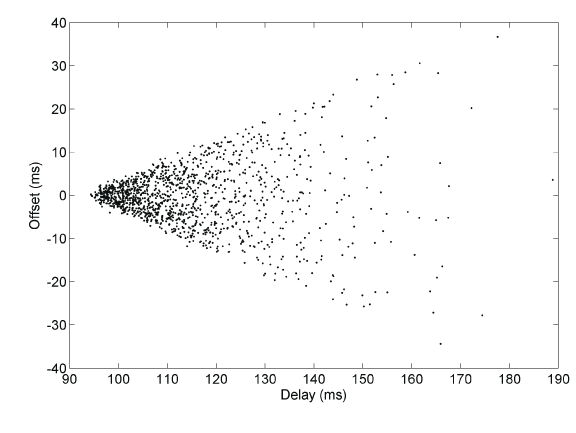
\includegraphics[width=0.5\textwidth]{figures/clock_filter.png}
    \caption{Wedge Scattergram}
    \label{fig:clock_filter}
\end{figure}


% fig:clock_filter

Based on the result we got from Figure~\ref{fig:clock_filter}, clock filter
algorithm first sorts the samples by their delay. If the first sample is later
than the last sample we selected, it is selected; otherwise nothing more
happens. This mechanism guarantees that one sample will only be used at most
once.

After the selection, the offset $\theta$ and delay $\delta$ of the sample
become peer statistics with the same names. The sorted samples are indexed from
0 to 7 from the one with the lowest delay to the one with highest. Here
$\varepsilon_i$ indicates the dispersion of the sample with index $i$. We
calculate peer dispersion $\varepsilon$ by:
\begin{equation}
    \varepsilon = \sum^{7}_{i=0} \frac{\varepsilon_i}{2^{(i+1)}}
    \label{eq:peer_dispersion}
\end{equation}
The peer jitter $\varphi$ is calculated by:
\begin{equation}
    \varphi = \sqrt{\frac{1}{n-1} \sum^{n-1}_{j=1} (\theta_0 - \theta_j)^2}
    \label{eq:peer_jitter}
\end{equation}
where $n$ is the number of valid samples in the shift register ($n > 1$).
The peer jitter is the root-mean-square (RMS) of differences between sample
offsets and the sample offset of selected sample, ``it represents the nominal
error in estimating the offset''~\cite{rfc5905}. A larger jitter indicates
that the offset varies more, in that case, we can consider that there may be
some problem with the server and/or the connection, since the offset should not
change much if we did not adjust client's system clock by a large amount.

\subsection{Huff-n'-puff filter}%
\label{sub:huff_n_puff_filter}
Now we are going to look at Figure~\ref{fig:clock_filter} closely. In the
figure, ``there are two limb lines with at slope $\pm0.5$, representing the
limits of sample variation''~\cite{clock_filter}.
The variation of offset is caused by the asymmetric delay, and it is actually
an error.

Figure~\ref{fig:huff_n_puff1} shows the relationship between delay and offset
error.  Figure~\ref{subfig:best_case} shows the best case where the delays are
symmetric. In this case, the middle points which are indicated by the ends of
dash line (other two figures are the same) are at the same time. As we
mentioned in Section~\ref{sub:statistics_calculation}, the calculation in
Equation~\ref{eq:offset_def} is correct. 

% figures/huff_n_puff1.tex

\begin{figure}[htpb]
\begin{center}
\subfloat[Best case]{
\begin{tikzpicture}[scale=0.73, transform shape,
        textnode/.style={rectangle, very thick, minimum
        size=10mm, minimum width=20mm, align=center},
        border/.style={draw=black, dashed, very thick},
        arrow/.style={-latex, ultra thick},
    ]
    % server
    \node[textnode]  (s)                        {Server};
    \draw[arrow]     (s) -- ($(s) + (9,0)$);

    % client
    \node[textnode]  (c)    [below=20mm of s]   {Client};
    \draw[arrow]     (c) -- ($(c) + (9,0)$);

    % communications
    \draw[arrow]     ($(c) + (3, 0)$) -- ($(s) + (3.5, 0)$);
    \draw[arrow]     ($(s) + (6.5, 0)$) -- ($(c) + (7, 0)$);

    % dash line
    \draw[border]    ($(s) + (5, 0)$) -- ($(c) + (5, 0)$);
\end{tikzpicture}
\label{subfig:best_case}
}
\subfloat[Normal case]{
\begin{tikzpicture}[scale=0.7, transform shape,
        textnode/.style={rectangle, very thick, minimum
        size=10mm, minimum width=20mm, align=center},
        border/.style={draw=black, dashed, very thick},
        arrow/.style={-latex, ultra thick},
    ]
    % server
    \node[textnode]  (s)                        {Server};
    \draw[arrow]     (s) -- ($(s) + (9.5,0)$);

    % client
    \node[textnode]  (c)    [below=20mm of s]   {Client};
    \draw[arrow]     (c) -- ($(c) + (9.5,0)$);

    % communications
    \draw[arrow]     ($(c) + (3, 0)$) -- ($(s) + (4, 0)$);
    \draw[arrow]     ($(s) + (6, 0)$) -- ($(c) + (7.5, 0)$);

    % dash line
    \draw[border]    ($(s) + (5, 0)$) -- ($(c) + (5.25, 0)$);
\end{tikzpicture}
\label{subfig:normal_case}
}

\subfloat[Extremely asymmetric case]{
\begin{tikzpicture}[scale=0.7, transform shape,
        textnode/.style={rectangle, very thick, minimum
        size=10mm, minimum width=20mm, align=center},
        border/.style={draw=black, dashed, very thick},
        arrow/.style={-latex, ultra thick},
    ]
    % server
    \node[textnode]  (s)                        {Server};
    \draw[arrow]     (s) -- ($(s) + (10,0)$);

    % client
    \node[textnode]  (c)    [below=20mm of s]   {Client};
    \draw[arrow]     (c) -- ($(c) + (10,0)$);

    % communications
    \draw[arrow]     ($(c) + (3, 0)$) -- ($(s) + (3, 0)$);
    \draw[arrow]     ($(s) + (5, 0)$) -- ($(c) + (7.5, 0)$);

    % dash line
    \draw[border]    ($(s) + (4, 0)$) -- ($(c) + (5.25, 0)$);
    \draw[border]    ($(s) + (4, 0)$) -- ($(c) + (4, 0)$);

    % labels
    \node[textnode] at ($(c) + (3, -0.5)$)      {$T_0$};
    \node[textnode] at ($(s) + (3, 0.5)$)       {$T_1$};
    \node[textnode] at ($(s) + (5, 0.5)$)       {$T_2$};
    \node[textnode] at ($(c) + (7.5, -0.5)$)    {$T_3$};
    \node[textnode] at ($(s) + (4, 0.5)$)       {$T_4$};
    \node[textnode] at ($(c) + (5.25, -0.5)$)   {$T_5$};
    \node[textnode] at ($(c) + (4, -0.5)$)      {$T_6$};

\end{tikzpicture}
\label{subfig:extremely_asymmetric_case}
}
\end{center}
\caption{The relationship between delay and offset variance}
\label{fig:huff_n_puff1}
\end{figure}



% fig:huff_n_puff1

In Figure~\ref{subfig:normal_case}, it is the normal case, the delays are
slightly different, which makes the middle points slightly different as well.
This difference leads an error of offset.

In Figure~\ref{subfig:extremely_asymmetric_case}, it represents the extremely
asymmetric case, where there is no upload delay and the download delay is
relatively large. Assume $T_6$ and $T_4$ are captured in the same time, the
error of offset is the difference between $T_5$ and $T_6$. We can prove that it
is equal to $-\frac{1}{2}\delta$. In another case, if the upload delay is
relatively large and the download delay is zero, the error is equal to
$\frac{1}{2}\delta$. Note that these cases are the situations when the error is
maximum.

With this analysis, we know that the slope $\pm0.5$ is not determined by
experiment, but is calculated in theory and we know the variation of offset is
actually error, which is the reason that we select the sample with smallest
delay, which leads to smallest offset error.

The clock filter algorithm works best when there is a symmetric delay, as
Figure~\ref{fig:clock_filter} shows. It is also mentioned that the errors due
to asymmetric delay are almost unable to be corrected. However, huff-n'-puff
filter is used here to attenuate the errors.

Figure~\ref{fig:huff_n_puff2} shows the scattergram like
Figure~\ref{fig:huff_n_puff1}, but the network delay is much asymmetric. From
the figure, we find that the samples are close to the upper limb line, which
indicates that the offset error is positive. This means that the upload delay
is larger than the download delay. However, the document in~\cite{huff_n_puff}
shows the opposite opinion, which is wrong. By applying huff-n'-puff filter,
we can do the following stuff:
\begin{itemize}
    \item 
        Remember the recent sample with lowest delay where ``recent'' usually
        means recent hours. The offset and delay of the sample are denoted by 
        $\theta_0$ and $\delta_0$. Note that the sample is near the apex.
    \item 
        For a coming new sample whose offset and delay are $\theta_i$ and
        $\delta_i$, we keep its delay value and adjust offset by:
        \begin{equation}
            \theta = 
            \begin{cases}
                \displaystyle
                \theta_i - \frac{\delta_i - \delta_0}{2}, &\text{ if }\theta_i
                > \theta_0\\
                \displaystyle
                \theta_i + \frac{\delta_i - \delta_0}{2}, &\text{ if }\theta_i
                < \theta_0\\
            \end{cases}
            \label{eq:huff_n_puff}
        \end{equation}
\end{itemize}

% figures/huff_n_puff2.tex

\begin{figure}[htb]
    \centering
    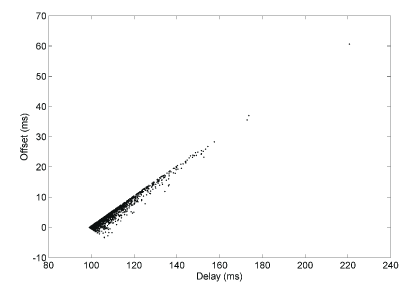
\includegraphics[width=0.8\textwidth]{figures/huff_n_puff.png}
    \caption{Huff-n'-puff Wedge Scattergram}
    \label{fig:huff_n_puff2}
\end{figure}


% fig:huff_n_puff2

Note that this adjustment is actually moving the sample points close to the
horizontal line which goes through the point $(\delta_0, \theta_0)$, if the
samples are near the upper limb line, as Figure~\ref{fig:huff_n_puff2} shows.
It is also said that it is less effective and will lead to significant errors
when a large amount of samples are in the area between the limb
lines.~\cite{huff_n_puff} If the practice situation is like
Figure~\ref{fig:huff_n_puff2}, the adjustment works fine, since it can avoid
the variation of offset which can be considered as error.

%\subsection{Reachability detection}%
%\label{sub:reachability_detection}
% https://docs.ntpsec.org/latest/stats.html
% redbook

\section{Poll processes}%
\label{sec:poll_processes}
As mentioned in Section~\ref{sec:peer_poll_overview}, poll processes are
designed to control the interval of communications in order to get sufficient
data without making servers too busy. 

The key part of poll process it the time constant $T_c$ and its relative 
exponent $\uptau$ where $T_c = 2 ^ {\uptau}$. A client send poll request to
each server with a \emph{poll interval} of $T_c$ seconds. $\uptau$ is a whole
number and is called the \emph{poll exponent}, which ranges from 4 to
17~\cite{rfc5905}.

$T_c$ and $\uptau$ are maintained by the clock discipline process. We will
discuss it later in Chapter~\ref{cha:clock_discipline_process}.

There are two options: \verb|BURST| and \verb|IBURST|. With the \verb|BURST|
option, instead of sending one request at each poll interval, the poll
process sends 8 packets. The intervals between packets are 2s. With the
\verb|IBURST| option, when a server is unreachable, it sends 8 packets at 2-s
intervals. The \verb|IBURST| option is used to reduce the synchronization
time at initial starts up while the \verb|BURST| option can reduce noise at
long poll intervals~\cite{poll_process}.

